% Options for packages loaded elsewhere
\PassOptionsToPackage{unicode}{hyperref}
\PassOptionsToPackage{hyphens}{url}
\PassOptionsToPackage{dvipsnames,svgnames,x11names}{xcolor}
%
\documentclass[
  english,
]{article}
\usepackage{amsmath,amssymb}
\usepackage{lmodern}
\usepackage{setspace}
\usepackage{iftex}
\ifPDFTeX
  \usepackage[T1]{fontenc}
  \usepackage[utf8]{inputenc}
  \usepackage{textcomp} % provide euro and other symbols
\else % if luatex or xetex
  \usepackage{unicode-math}
  \defaultfontfeatures{Scale=MatchLowercase}
  \defaultfontfeatures[\rmfamily]{Ligatures=TeX,Scale=1}
\fi
% Use upquote if available, for straight quotes in verbatim environments
\IfFileExists{upquote.sty}{\usepackage{upquote}}{}
\IfFileExists{microtype.sty}{% use microtype if available
  \usepackage[]{microtype}
  \UseMicrotypeSet[protrusion]{basicmath} % disable protrusion for tt fonts
}{}
\makeatletter
\@ifundefined{KOMAClassName}{% if non-KOMA class
  \IfFileExists{parskip.sty}{%
    \usepackage{parskip}
  }{% else
    \setlength{\parindent}{0pt}
    \setlength{\parskip}{6pt plus 2pt minus 1pt}}
}{% if KOMA class
  \KOMAoptions{parskip=half}}
\makeatother
\usepackage{xcolor}
\IfFileExists{xurl.sty}{\usepackage{xurl}}{} % add URL line breaks if available
\IfFileExists{bookmark.sty}{\usepackage{bookmark}}{\usepackage{hyperref}}
\hypersetup{
  pdflang={en},
  colorlinks=true,
  linkcolor={blue},
  filecolor={Maroon},
  citecolor={blue},
  urlcolor={blue},
  pdfcreator={LaTeX via pandoc}}
\urlstyle{same} % disable monospaced font for URLs
\usepackage[margin=1.25in]{geometry}
\usepackage{longtable,booktabs,array}
\usepackage{calc} % for calculating minipage widths
% Correct order of tables after \paragraph or \subparagraph
\usepackage{etoolbox}
\makeatletter
\patchcmd\longtable{\par}{\if@noskipsec\mbox{}\fi\par}{}{}
\makeatother
% Allow footnotes in longtable head/foot
\usepackage{footnote} % For some unknown reason, footnotehyper clashes with French
\makesavenoteenv{longtable}
\usepackage{graphicx}
\makeatletter
\def\maxwidth{\ifdim\Gin@nat@width>\linewidth\linewidth\else\Gin@nat@width\fi}
\def\maxheight{\ifdim\Gin@nat@height>\textheight\textheight\else\Gin@nat@height\fi}
\makeatother
% Scale images if necessary, so that they will not overflow the page
% margins by default, and it is still possible to overwrite the defaults
% using explicit options in \includegraphics[width, height, ...]{}
\setkeys{Gin}{width=\maxwidth,height=\maxheight,keepaspectratio}
% Set default figure placement to htbp
\makeatletter
\def\fps@figure{htbp}
\makeatother
\setlength{\emergencystretch}{3em} % prevent overfull lines
\providecommand{\tightlist}{%
  \setlength{\itemsep}{0pt}\setlength{\parskip}{0pt}}
\setcounter{secnumdepth}{-\maxdimen} % remove section numbering
\newlength{\cslhangindent}
\setlength{\cslhangindent}{1.5em}
\newlength{\csllabelwidth}
\setlength{\csllabelwidth}{3em}
\newlength{\cslentryspacingunit} % times entry-spacing
\setlength{\cslentryspacingunit}{\parskip}
\newenvironment{CSLReferences}[2] % #1 hanging-ident, #2 entry spacing
 {% dont indent paragraphs
  \setlength{\parindent}{0pt}
  % turn on hanging indent if param 1 is 1
  \ifodd #1
  \let\oldpar\par
  \def\par{\hangindent=\cslhangindent\oldpar}
  \fi
  % set entry spacing
  \setlength{\parskip}{#2\cslentryspacingunit}
 }%
 {}
\usepackage{calc}
\newcommand{\CSLBlock}[1]{#1\hfill\break}
\newcommand{\CSLLeftMargin}[1]{\parbox[t]{\csllabelwidth}{#1}}
\newcommand{\CSLRightInline}[1]{\parbox[t]{\linewidth - \csllabelwidth}{#1}\break}
\newcommand{\CSLIndent}[1]{\hspace{\cslhangindent}#1}

%%%%%%%% START HEADER PARTIAL %%%%%%%%%%%%

% Formatting of tables & knitr::kable and kableExtra functionality
\usepackage{float}
\usepackage{colortbl}
\usepackage{pdflscape}
\usepackage{tabu}
\usepackage{threeparttable}

% Line numbering

% endfloat stuff

% fancyhdr pagestyle

% Environment for keywords
\makeatletter
\newcommand\keywordsname{Keywords}
\newenvironment*{keywords}[1][\keywordsname]{\if@twocolumn \else \small \quotation \fi \begin{center} \textbf{\textit{#1} \\}}{\end{center}\if@twocolumn \else \small \endquotation \fi}
\newenvironment*{keywordsinline}[1][\keywordsname]{\if@twocolumn \else \small \quotation \fi \begin{center} \textbf{\textit{#1}: }}{\end{center}\if@twocolumn \else \small \endquotation \fi}
\makeatother

% Environment for abstract that takes new abstract name
\newenvironment{renameableabstract}[1][\abstractname]{\let\oldabstractname\abstractname \renewcommand{\abstractname}{#1} \begin{abstract}}{\end{abstract} \renewcommand{\abstractname}{\oldabstractname}}

%%%%%%%% END HEADER PARTIAL %%%%%%%%%%%%

\usepackage{tikz}
\usetikzlibrary{angles,positioning,arrows.meta, quotes, shapes, shapes.geometric}
\usepackage{graphicx}
\usepackage{booktabs}
\usepackage{longtable}
\usepackage{array}
\usepackage{multirow}
\usepackage{wrapfig}
\usepackage{float}
\usepackage{colortbl}
\usepackage{pdflscape}
\usepackage{tabu}
\usepackage{threeparttable}
\usepackage{threeparttablex}
\usepackage[normalem]{ulem}
\usepackage{makecell}
\usepackage{xcolor}
\ifXeTeX
  % Load polyglossia as late as possible: uses bidi with RTL langages (e.g. Hebrew, Arabic)
  \usepackage{polyglossia}
  \setmainlanguage[]{}
\else
  \usepackage[english,main=english]{babel}
% get rid of language-specific shorthands (see #6817):
\let\LanguageShortHands\languageshorthands
\def\languageshorthands#1{}
\fi
\ifLuaTeX
  \usepackage{selnolig}  % disable illegal ligatures
\fi

\title{Interaction structure constrains\\
the emergence of conventions in group communication}

%%%%%%% START AUTHOR PARTIAL %%%%%%%%%%%%%%%

%%%%% Authors, affiliations and author notes stuff %%%%%

% Macros for creating and referencing stored reference
\makeatletter
\def\MyNewLabel#1#2#3{\expandafter\gdef\csname #1@#2\endcsname{#3}}

\def\MyRef#1#2{\@ifundefined{#1@#2}{???}{\csname #1@#2\endcsname}}

\newcommand*\ifcounter[1]{%
  \ifcsname c@#1\endcsname
    \expandafter\@firstoftwo
  \else
    \expandafter\@secondoftwo
  \fi
}
\makeatother

% Create labels for Addresses if the are given by code
\MyNewLabel{ADDRTXT}{Stanford}{Stanford University}
\MyNewLabel{ADDRTXT}{Princeton}{Princeton University}

% Create labels for Footnotes if they are given by code
\MyNewLabel{ANOTETXT}{corresp}{Corresponding author. Email: \href{mailto:vboyce@stanford.edu}{\nolinkurl{vboyce@stanford.edu}}}

%%% Special footnotes for addresses and author footnotes
\usepackage{bigfoot}
\DeclareNewFootnote{Addr}[arabic] % Only used for NOT authblk
\DeclareNewFootnote{ANote}[fnsymbol]

%%% Address and author notes as a function of format %%%
 % Use authblk for affiliations %%%%%%%%%%%
\usepackage{authblk}

% Always separate by commas
\renewcommand\Authsep{, }
\renewcommand\Authand{, }
\renewcommand\Authands{, }

% Counter for addresses and footnotes
\newcounter{addrcnt}

% thanks definition that doesnt produce superscript marks
\makeatletter
\newcommand*\createaddrlblbycode[1]{%
  \ifcounter{ADDRLBL@#1}
    {}
    {\refstepcounter{addrcnt}\newcounter{ADDRLBL@#1}\setcounter{ADDRLBL@#1}{\value{addrcnt}}}%
}

\newcommand*\addrlblbycode[1]{\arabic{ADDRLBL@#1}}

\newcommand*\addrbycode[1]{%
  \ifcounter{ADDR@#1}
    {}
    {\newcounter{ADDR@#1}%
     \affil[\addrlblbycode{#1}]{\MyRef{ADDRTXT}{#1}}}%
}

\newcommand*\createanotelblbycode[1]{%
  \ifcounter{ANOTELBL@#1}
    {}
    {\refstepcounter{footnoteANote}\newcounter{ANOTELBL@#1}\setcounter{ANOTELBL@#1}{\value{footnoteANote}}}%
}

\newcommand*\anotelblbycode[1]{\fnsymbol{ANOTELBL@#1}}

\newcommand*\anotebycode[1]{%
  \ifcounter{ANOTE@#1}
    {}
    {\newcounter{ANOTE@#1}%
     \footnotetextANote[\value{ANOTELBL@#1}]{\MyRef{ANOTETXT}{#1}}}%
}
\makeatother


\createaddrlblbycode{Stanford}


\createanotelblbycode{corresp}

\author[%
\addrlblbycode{Stanford}%
,%
$\anotelblbycode{corresp}$%
]{Veronica Boyce}

\addrbycode{Stanford}


\createaddrlblbycode{University of Wisconsin--Madison}



\author[%
\addrlblbycode{University of Wisconsin--Madison}%
]{Robert Hawkins}

\addrbycode{University of Wisconsin--Madison}


\createaddrlblbycode{Stanford}



\author[%
\addrlblbycode{Stanford}%
]{Noah D. Goodman}

\addrbycode{Stanford}


\createaddrlblbycode{Stanford}



\author[%
\addrlblbycode{Stanford}%
]{Michael C. Frank}

\addrbycode{Stanford}


%endif(authblk)

%%%%%%%%% END AUTHOR PARTIAL %%%%%%%%

\date{}

\begin{document}
\maketitle

%%%%%%%%%% START AFTER TITLE PARTIAL %%%%%%%%%%%%%
\anotebycode{corresp}


%%%%%%%%%% END AFTER TITLE PARTIAL %%%%%%%%%%%%%


\setstretch{1}
\begin{otherlanguage}{english}

\begin{abstract}
Real-world communication frequently requires speakers to address more than one listener at once, yet most psycholinguistic research focuses on one-on-one communication.
As the audience size grows, speakers face new challenges that do not arise in dyads.
They must consider multiple perspectives and weigh multiple sources of feedback to build shared understanding.
Here, we ask which properties of the group's \emph{interaction structure} facilitates successful communication.
We used a repeated reference game paradigm in which directors instructed between one and five matchers to choose specific targets out of a set of abstract figures.
Across 313 games (\(N=1,319\) participants), we manipulated several key constraints on the group's interaction, including the amount of feedback that matchers could give to directors and the availability of interaction between matchers.
Larger groups suffered disproportionately under interaction constraints, but in less-constrained interaction structures (``thick channels''), \textbf{they were able to converge on efficient shared conventions as effectively as smaller groups.}
Overall, these results shed new light on the core structural factors that enable communication to thrive in larger groups.

\end{abstract}

\end{otherlanguage}

\hypertarget{introduction}{%
\section{Introduction}\label{introduction}}

Much of human social life revolves around communication in groups.
At school, teachers address large classrooms of children (\protect\hyperlink{ref-cazden1988classroom}{Cazden 1988}); at home, we chat with groups of friends and family members over dinner (\protect\hyperlink{ref-tannen2005conversational}{Tannen 2005}); and at work, we attend meetings with colleagues and managers (\protect\hyperlink{ref-caplow1957organizational}{Caplow 1957}, \protect\hyperlink{ref-zack1993interactivity}{Zack 1993}).
Such settings present considerable challenges that do not arise in the purely two-party (dyadic) settings typically studied in psychology (\protect\hyperlink{ref-traum2004}{Traum 2004}, \protect\hyperlink{ref-ginzburg2005}{Ginzburg \& Fernandez 2005}, \protect\hyperlink{ref-branigan2006}{Branigan 2006}).
For example, speakers need to account for the fact that different listeners in the group may have different mental states or levels of background understanding (\protect\hyperlink{ref-horton2002}{Horton \& Gerrig 2002}, \protect\hyperlink{ref-weber2003}{Weber \& Camerer 2003}, \protect\hyperlink{ref-horton2005}{Horton \& Gerrig 2005}, \protect\hyperlink{ref-fox-tree2013}{Fox Tree \& Clark 2013}, \protect\hyperlink{ref-yoon2014}{Yoon \& Brown-Schmidt 2014}, \protect\hyperlink{ref-yoon2018}{2018}), while listeners must account for the fact that utterances are not necessarily tailored to them (\protect\hyperlink{ref-carletta1998}{Carletta et al. 1998}, \protect\hyperlink{ref-fay2000}{Fay et al. 2000}, \protect\hyperlink{ref-metzing2003}{Metzing \& Brennan 2003}, \protect\hyperlink{ref-rogers2013}{Rogers et al. 2013}, \protect\hyperlink{ref-tolins2016}{Tolins \& Fox Tree 2016}, \protect\hyperlink{ref-cohngordon}{Cohn-Gordon et al. 2019}, \protect\hyperlink{ref-yoon2019}{Yoon \& Brown‐Schmidt 2019}).\footnote{\textbf{Throughout this paper, we use ``speaker'' and ``listener'' -- regardless of communication modality -- to refer to both the general conversation roles played by language producers and comprehenders as well as the the specific roles of describing and selecting targets in reference games of the type we study here.}}
What enables speakers and listeners to nevertheless overcome these challenges and navigate multi-party settings with relative ease?

One promising set of hypotheses centers on the group's \emph{interaction structure}, the set of constraints placed on the group's shared communication channel.
Many different aspects of interaction structure have been implicated in the effectiveness of dyadic communication, including the availability and quality of concurrent feedback (\protect\hyperlink{ref-krauss1966}{Krauss \& Weinheimer 1966}, \protect\hyperlink{ref-KraussBricker67_Delay}{Krauss \& Bricker 1967}, \protect\hyperlink{ref-kraut1982listener}{Kraut et al. 1982}), the bandwidth of the communication modality (\protect\hyperlink{ref-dewhirst1971influence}{Dewhirst 1971}, \protect\hyperlink{ref-KraussEtAl77}{Krauss et al. 1977}), and the group's access to a shared workspace (\protect\hyperlink{ref-clark2004speaking}{Clark \& Krych 2004}, \protect\hyperlink{ref-garrod2007foundations}{Garrod et al. 2007}).
Yet larger group introduce qualitatively different dimensions of interaction structure, leading to a large but often inconsistent body of findings even for these well-understood factors (\protect\hyperlink{ref-hiltz1986experiments}{Hiltz et al. 1986}, \protect\hyperlink{ref-swaab2012communication}{Swaab et al. 2012}).
While communication is generally expected to deteriorate as groups get larger (\protect\hyperlink{ref-seaman1997communication}{Seaman \& Basili 1997}, \protect\hyperlink{ref-macmillan_communication_2004}{MacMillan et al. 2004}), several factors that may slow such deterioration have been identified in qualitative work, each of which relates to the structural ``thickness'' of the feedback channel (\protect\hyperlink{ref-ahern1994effect}{Ahern 1994}, \protect\hyperlink{ref-parisi2005evaluating}{Parisi \& Brungart 2005}).

In this paper, we develop an experimental paradigm for evaluating the relative contribution of these factors: a \emph{multi-party repeated reference game.}
The ability to distinguish one particular entity from other possible entities, known as \emph{reference}, is one of the most primitive and ubiquitous functions of communication.
Reference games (\protect\hyperlink{ref-Wittgenstein1953}{Wittgenstein 1953}, \protect\hyperlink{ref-lewis1969convention}{Lewis 1969}) have been widely used to study dyadic communication under controlled conditions in the lab.
They provide a clear metric of communicative effectiveness: how many words are required before a listener successfully chooses a target image from a context of distractors?
\emph{Repeated} reference games, where the same target images appear multiple times in succession, were introduced to examine how interlocutors establish shared reference in the absence of conventional labels (\protect\hyperlink{ref-krauss1964}{Krauss \& Weinheimer 1964}, \protect\hyperlink{ref-clark1986}{Clark \& Wilkes-Gibbs 1986}).
At the beginning of the game, long and costly descriptions are typically required to succeed.
A key finding, however, is that dyads become increasingly efficient over the course of interaction.
Later utterances require fewer words, but also become more impenetrable to outsiders (\protect\hyperlink{ref-schober1989}{Schober \& Clark 1989}, \protect\hyperlink{ref-wilkes1992coordinating}{Wilkes-Gibbs \& Clark 1992}).

In principle, repeated reference games provide a strong operationalization of communicative effectiveness for the problem of multi-party communication: speakers must simultaneously achieve shared reference with multiple listeners.
However, empirically studying multi-party communication raises a number of difficulties in practice.
A much larger pool of participants must be recruited to achieve sufficient power at the relevant unit of analysis -- the group -- spanning a very high-dimensional space of possible parameter settings (\protect\hyperlink{ref-almaatouq2022}{Almaatouq et al. 2022}).
We address this problem by drawing on recent technical advances that have made it newly possible to achieve such samples using an interactive web-based platform (\protect\hyperlink{ref-haber2019}{Haber et al. 2019}, \protect\hyperlink{ref-hawkins2023partners}{Hawkins et al. 2023}).
Repeated reference games in online, chat-based paradigms have closely replicated earlier results from face-to-face studies (\protect\hyperlink{ref-hawkins2020}{Hawkins et al. 2020}), and arguably more closely resemble the interfaces used by modern teams who increasingly communicate through group text threads or popular platforms like Slack or Discord.

We use the multi-party repeated reference game to explore effects of group size and interaction channel thickness through a series of three experiments. \textbf{Taken together, our findings illuminate the mechanisms of social interaction in larger groups and suggest design features that may ease the communicative overhead associated with larger groups in real-world settings.}

\begin{figure*}[t!]

{\centering 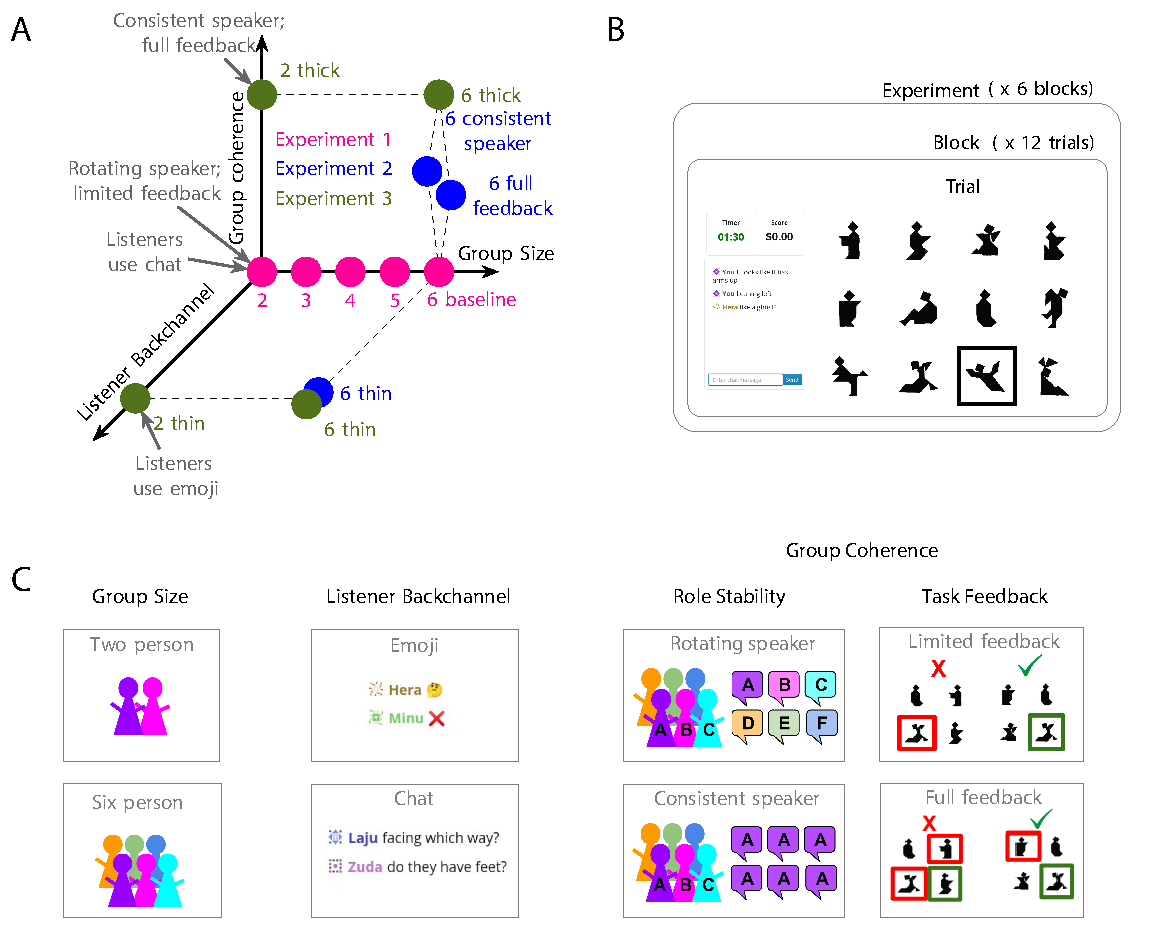
\includegraphics[width=1\linewidth]{fig1} 

}

\caption{(A) Participants played a repeated reference game in groups of size 2 to 6. On each trial, speakers described a target image to the listeners. Each image appeared once per block for six blocks. (B) Diagram of the experimental space. Experiments varied along 3 dimensions: Group size, group coherence, and listener backchannel. (C) Schematic of the axes we manipulated. Experiment 1 (pink) varied group size from 2 to 6 players while holding group coherence and backchannel constant. Experiment 2 (blue) held group size constant at 6 and manipulated the other dimensions. Experiment 3 (green) tested 4 corners of the space, crossing group size (2 vs. 6 players) with the thickness of interaction structure (high vs. low coherence and backchannel).}\label{fig:diagram}
\end{figure*}

\hypertarget{results}{%
\section{Results}\label{results}}

We recruited 1319 participants through Prolific, an online crowd-sourcing platform.
Participants were organized into 313 groups of size two to six for a communication game (Figure \ref{fig:behavioral}A).
On each trial, everyone in the group was shown a gallery of 12 tangram images (\protect\hyperlink{ref-clark1986}{Clark \& Wilkes-Gibbs 1986}, \protect\hyperlink{ref-hawkins2020}{Hawkins et al. 2020}, \protect\hyperlink{ref-ji2022abstract}{Ji et al. 2022}).
One player was designated the \emph{speaker} and the others were designated the \emph{listeners}.
The speaker was asked to use a chat box interface to describe a privately indicated \emph{target} image.
After all listeners guessed which of the 12 images was the target, they received task feedback and proceeded to the next trial.
The game consisted of 72 trials structured into 6 repetition blocks, where each image appeared as the target exactly once per block.

We manipulated the interaction structure of this game across 11 distinct conditions in 3 distinct pre-registered experiments (Figure \ref{fig:behavioral}B).
We systematically sampled points along four dimensions parameterizing different aspects of the interaction space.
We manipulated \emph{group size} (ranging from two to six), \emph{role stability} (whether or not participants took turns in the speaker role), richness of \emph{task feedback} (whether or not listeners were able to see each other's responses), and richness of the \emph{listener backchannel} (whether listeners were able to freely respond through a chatbox or could only use emojis; Figure \ref{fig:behavioral}C).
Other factors, such as the set of stimuli and background knowledge about one's partners, were held constant across games.

Experiment 1 investigated how performance scaled with group size.
Based on prior qualitative work, we predicted that larger groups face a more challenging coordination problem.
We continuously varied the number of players from 2 to 6 while keeping other factors constant.
For these conditions, the speaker role rotated after each block, so that all players had at least one turn as speaker.
Listeners had access to an unrestricted chat box, but only received binary task feedback about whether their individual selection was correct without revealing others' selections or the intended target.

Experiment 2 explored the role of interaction structure purely within the most challenging 6-player groups.
We manipulated two factors that we expected to increase group coherence and improve performance.
First, we maintained a consistent speaker rather than a rotating speaker, such that the same individual has the opportunity to aggregate feedback across trials and track which listeners are struggling which which targets.
Second, we gave the group of listeners full feedback about what every other member of the group had selected, and we showed the intended target.
We also manipulated a factor that we expected to interfere with the ability to establish mutual understanding and thus impede performance.
In the limited backchannel condition, listeners were limited to four discrete emojis (green check, thinking face, red x, and laughing-crying face) that could convey simple valence and level of comprehension, but not any referential content.

Experiment 3 crossed the extremes of group size from experiment 1 (2 vs.~6 people) with the extremes of group interactions from Experiment 2 (\emph{thick} vs.~\emph{thin} interaction structure).
In the \emph{thick} condition, we maintained a consistent speaker, gave all listeners full task feedback, and allowed them to freely use a chat box.
In the \emph{thin} condition, we forced the speaker to rotate on each block, restricted feedback to their own binary correctness, and restricted the backchannel to the four emojis.
Note that the 2-player thick game most closely resembles the design of classic repeated reference games (\protect\hyperlink{ref-clark1986}{Clark \& Wilkes-Gibbs 1986}, \protect\hyperlink{ref-hawkins2020}{Hawkins et al. 2020}).

\begin{figure*}[t!]

{\centering \includegraphics[width=1\linewidth]{figs/behavioral-1} 

}

\caption{Behavioral results across all three experiments. (A-C). Listener accuracy at selecting the target image. Small dots are per game, per block means. Smooths are binomial fit lines.  (D-F). Number of words said by the speaker each trial. Small dots are per game, per block means. Smooths are quadratic fit lines. Y-axes are truncated, and a few outliers points are not visible. **(TODO check ordering of legends!)**}\label{fig:behavioral}
\end{figure*}

\hypertarget{group-performance}{%
\subsection{Group Performance}\label{group-performance}}

We characterize group performance along two complementary metrics: (1) listener accuracy and (2) speaker efficiency.
Listener accuracy is given by the percent of listeners on each trial who successfully identify the target referent from the speaker's description.
Speaker efficiency is given by the number of words produced by the speaker to achieve that degree of listener accuracy in the group.
The degree to which speakers are able to communicate more efficiently without negatively impacting listener accuracy is indicative of convergence on a more effective shared communication protocol within the group.

\hypertarget{communicative-success-improves-across-conditions}{%
\subsubsection{Communicative success improves across conditions}\label{communicative-success-improves-across-conditions}}

We begin by examining the impact of interaction structure on referential success, the ability to correctly transmit the intended target to all listeners (Figure \ref{fig:behavioral}A-C).
We predicted that larger groups would struggle under thinner interaction structures, but that thicker interaction structures would ease some of the challenges associated with multi-listener communication.
To test these effects, we constructed a series of 5 logistic mixed-effects regression models predicting accuracy as a function of the manipulated variables, repetition block, and their interactions (separate models were run for experiment 1, each condition in experiment 2, and experiment 3).

First, we observed strong positive effects of repetition block, indicating improved performance over time in each condition (Figure \ref{fig:behavioral}A-C, SI Tables 2-6).
Second, we examined the \emph{initial} accuracy as an indicator of the challenges facing groups under different conditions.
Although the continuous measure of group size in Experiment 1 did not have a strong effect on initial accuracy (Figure \ref{fig:behavioral}A, SI Table 2), 6-player thick games had lower initial accuracy than 2-player thick games (Figure \ref{fig:behavioral}C, \(\beta=-0.64,\:95\%\:\mathrm{CrI}=[-1.05, -0.25]\)). Among 6-player games, initial accuracy was also higher when the speaker was consistent or listeners received full feedback than for games with a thin feedback channel (Figure \ref{fig:behavioral}B, SI Tables 3-5).

Third, we examined the interaction between condition and repetition block to test whether interaction structure impacts the rate of improvement.
Again, there was no reliable effect of group size in Experiment 1 (SI Table 2), although 6-player thick games were slower to improve than 2-player thick games (\(\beta=-0.34,\:95\%\:\mathrm{CrI}=[-0.43, -0.25]\)).
Among large groups in Experiment 2, improvement rates were higher for consistent speaker games and full feedback games than for thin games (Figure \ref{fig:behavioral}B, SI Tables 3-5).
The difference in improvement rates between thick and thin 2-player games was not reliable nor was their a reliable interaction between group size and thickness on improvement rate (SI Table 6).

\textbf{TODO this is now truthful, but not very punchy}In sum, participants may struggle more in larger groups, but these effects are not consistently reliable, perhaps due to to inter-group variability. Regardless of group size and interaction structure, groups were far above chance and improved over the course of the game.

\hypertarget{larger-groups-require-more-information.}{%
\subsubsection{Larger groups require more information.}\label{larger-groups-require-more-information.}}

After establishing that groups were able to communicate the targets successfully, we turned to the challenges faced by speakers when deciding how much information to provide.
Specifically, we predicted that larger and more heterogeneous groups may initially require more information, but that thicker interaction structure may similarly allow speakers to communicate more effectively over time.
We tested these predictions using linear mixed-effects models predicting the number of words a speaker produced on each trial as a function of condition and block. These models included everything the speaker said, including after listener contributions (for similar models of just speaker's utterances before any listener contribution, see SI Tables 15-18).

First, as predicted, speakers in larger groups used longer descriptions at the outset than speakers in smaller groups (Figure \ref{fig:behavioral}D-F). This held for the continuous measure of group size for Experiment 1 (\(\beta=1.6,\:95\%\:\mathrm{CrI}=[0.62, 2.6]\)) and the 2-person versus 6-person groups in Experiment 3 (\(\beta=7.51,\:95\%\:\mathrm{CrI}=[3.63, 11.3]\)).
Second, although communicative efficiency improved at a similar rate across group size in Experiment 1 (\(\beta=-0.09,\:95\%\:\mathrm{CrI}=[-0.37, 0.18]\)), in Experiment 3, larger groups reduced faster than smaller ones in Experiment 3 (\(\beta=-1.22,\:95\%\:\mathrm{CrI}=[-2.06, -0.29]\)). However, the faster reduction did not fully make up for the initial longer utterances, so across both experiments smaller games tended to use shorter descriptions.

Interaction structure did not show a consistent effect on utterance length. While thin 6 player games showed a flatter reduction trajectory than thicker 6 player games in Experiment 2 (SI Tables 8-10), there was not a reliable effect of game thickness on reduction in Experiment 3 for either smaller or larger groups (SI Table 11).

Overall, speakers on average decreased their descriptions by a few words each repetition block, ranging from -5.31, (\(95\%\:\mathrm{CrI}=[-6.35, -4.3]\)) words in 6-player consistent speaker to -2.1, (\(95\%\:\mathrm{CrI}=[-3.37, -1.12]\)) words in 6-player thin.

\textbf{TODO punch back up again?}In sum, while larger groups of listeners initially require more information from the speaker, all conditions allowed groups to reduce to more efficient referential conventions.

\hypertarget{larger-groups-use-backchannels-more}{%
\subsubsection{Larger groups use backchannels more}\label{larger-groups-use-backchannels-more}}

Finally, we examine the back-and-forth interactions between the speaker and the group of listeners.
The backchannel allows listeners to actively provide feedback and seek clarification about the speaker's referring expressions. An example transcript from a game where listeners contributed in various ways is in Table \ref{tab:listener-example}.
We predicted that larger groups would initially rely more heavily on lateral peer interactions, the ability to deliberate and assist one another.
However, as groups converged, we expected the use of these backchannels to decline.
To test these predictions, we constructed a logistic regression predicting the presence of listener utterances as a function of group size and block.

Overall, larger groups displayed a higher proportion of trials where at least one listener backchannel response was produced (Supplement Figure 2A, \(\beta=0.79,\:95\%\:\mathrm{CrI}=[0.58, 0.98]\)), which declined across blocks (\(\beta=-0.8,\:95\%\:\mathrm{CrI}=[-0.97, -0.62]\)).
This pattern is consistent with early listener involvement in establishing a common conceptualization by asking questions and offering alternative descriptions.
We found that emoji use in Experiment 3 followed similar trends (Supplement Figure 3).

\begin{table}[H]

\caption{\label{tab:listener-example}Example transcript of a 6-player group for Experiment 1 describing the same image each repetition. Listeners sometimes asked questions or offered clarifications, including in reference to prior descriptions.}
\centering
\begin{tabu} to \linewidth {>{\raggedright\arraybackslash}p{8em}>{\raggedright\arraybackslash}p{28em}}
\toprule
\addlinespace[0.3em]
\multicolumn{2}{l}{\textbf{Block 1}}\\
\hspace{1em}A (speaker) & classic ghost or man with his hands up\\
\hspace{1em}A (speaker) & slanted\\
\hspace{1em}A (speaker) & slanted to the left\\
\hspace{1em}D & slanted left? Right arm hanging out?\\
\hspace{1em}A (speaker) & both arms up\\
\hspace{1em}A (speaker) & and out\\
\hspace{1em}F & no \vphantom{1} legs\\
\hspace{1em}A (speaker) & no legs \textasciicircum{}\\
\addlinespace[0.3em]
\multicolumn{2}{l}{\textbf{Block 2}}\\
\hspace{1em}C (speaker) & whole body tilted to the left, as if falling over\\
\hspace{1em}C (speaker) & arms in air\\
\hspace{1em}D & Like a 1 legged exercise lunge though? Holding a medicine ball?\\
\hspace{1em}F & left side like an open wrench\\
\hspace{1em}C (speaker) & like a ghost falling over\\
\hspace{1em}F & no legs\\
\hspace{1em}D & Okayyyy Ghost. Got it\\
\addlinespace[0.3em]
\multicolumn{2}{l}{\textbf{Block 3}}\\
\hspace{1em}D (speaker) & The classic ghost. Arms are up in the air\\
\hspace{1em}D (speaker) & Whole body slanted left\\
\hspace{1em}F & both arms up not legs\\
\hspace{1em}D (speaker) & The right arm is further from the head than left\\
\hspace{1em}D (speaker) & No legs visible\\
\addlinespace[0.3em]
\multicolumn{2}{l}{\textbf{Block 4}}\\
\hspace{1em}B (speaker) & whole body slanting left with arms in the air\\
\hspace{1em}D & Classic ghost?\\
\addlinespace[0.3em]
\multicolumn{2}{l}{\textbf{Block 5}}\\
\hspace{1em}E (speaker) & slanted shadow or ghost, arms up, no feet\\
\addlinespace[0.3em]
\multicolumn{2}{l}{\textbf{Block 6}}\\
\hspace{1em}F (speaker) & classic ghost, both arms up, no legs, slanting back to the left\\
\bottomrule
\end{tabu}
\end{table}

\hypertarget{interim-summary}{%
\subsubsection{Interim summary}\label{interim-summary}}

We examined three metrics of communicative performance in groups of different sizes and interaction structures.
\textbf{Broadly, as groups get larger, speakers must provide more information and listeners must provide more feedback to achieve similar accuracy. However, thicker interaction structures ease the burdens of larger group sizes. Six-person groups can only approach the performance of two-person groups when listeners are free to ask specific clarifying questions and speakers are able to aggregate information across multiple repetition blocks.}

\hypertarget{linguistic-content}{%
\subsection{Linguistic Content}\label{linguistic-content}}

\begin{figure*}[t!]

{\centering 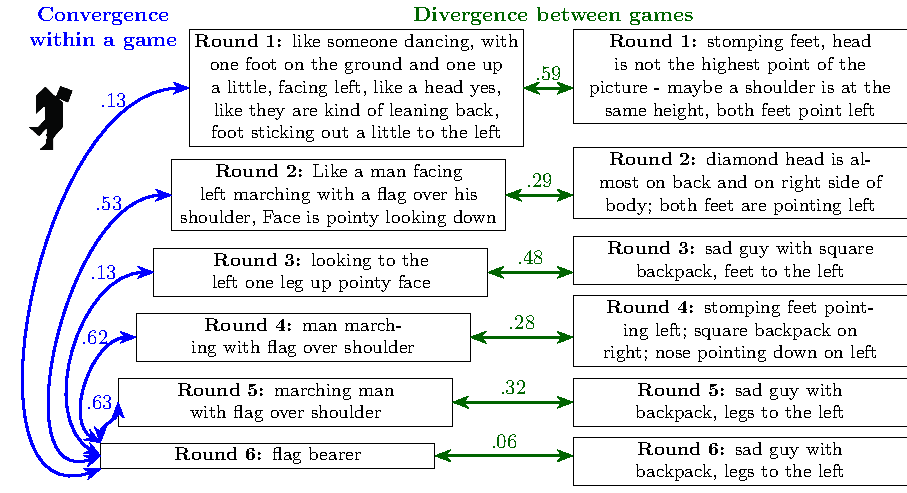
\includegraphics[width=1\linewidth]{sbert} 

}

\caption{Example utterances describing the shown tangram figure produced by two 3-player games in Experiment 1. To measure convergence within a game (blue), we measured the cosine similarity between SBERT embeddings of descriptions and the embedding of the round 6 utterance (taken to be the convention). Higher cosine similarity indicates more similar meaning. To measure divergence between games (green), we measured the similarity between embeddings of utterances from the same round across games.}\label{fig:sbert-diagram}
\end{figure*}

\textbf{In the previous sections, we explored the functional challenges facing multi-listener communication and the solutions afforded by thicker interaction structure.}
Here, we aim to better understand the mechanisms that make these solutions effective.
In particular, we explore the hypothesis that interaction structure affects performance by acting through a \emph{convention formation} process (\protect\hyperlink{ref-clark1986}{Clark \& Wilkes-Gibbs 1986}).
Under a recent models of convention formation (\protect\hyperlink{ref-hawkins2023partners}{Hawkins et al. 2023}), groups are able to leverage their shared history to coordinate on stable expectations about how to refer to particular images.
This model makes specific predictions about how interaction structure affects the ability to coordinate, in terms of the available feedback.

First, due to heterogeneity in the group -- 6 individuals who may have diverging conceptualizations --- a rational speaker should provide a strictly more detailed initial description to hedge against multiple possible misunderstandings, as we previously observed.
Second, all groups should display the characteristic dynamics of conventions: \emph{stability}, or convergence within group, and \emph{arbitrariness}, or divergence to multiple equilibria across groups.
Third, convergence should be faster when a single individual is consistently in the speaker role and when listeners are able to freely respond in natural language, as speakers are able to aggregate feedback about the effectiveness of their own utterances from block to block and also immediately correct specific misunderstandings within a given trial.

To assess the dynamics of speaker descriptions, we examine the \emph{semantic similarity} of descriptions within and across games.
We quantified description similarity by concatenating speaker messages together within a trial and embedding this description into a high-dimensional vector space using SBERT.
SBERT is a BERT-based sentence embedder designed to map semantically similar sentences to embeddings that are nearby in embedding space.
Semantically meaningful comparisons between sentences are made by taking pairwise cosine similarities between the embeddings (\protect\hyperlink{ref-reimers2019}{Reimers \& Gurevych 2019}).

To measure stability, or convergence within groups, we compared utterances from blocks one through five to the final (block six) description for the same image from the same game.
To measure arbitrariness, or divergence across groups, depending on group-specific history, we compared utterances produced by different speakers for the same image in the corresponding blocks.
Figure \ref{fig:sbert-diagram} illustrates these two measures with example concatenated utterances and their within-game and between-game cosine similarities.

\begin{figure*}[t!]

{\centering \includegraphics[width=1\linewidth]{figs/sbert-1} 

}

\caption{Language similarity results measured with pairwise cosine similarity between embeddings of two utterances. A-C. Convergence of descriptions within games as measured by similarity between an utterance from block 1-5 to the block 6 utterance in the same game for the same image. Dots are per-game averages, smooths are quadratic. D-F. Divergence of descriptions across games as measured by the similarity between two utterances produced for the same image by different groups in the same block. Dots are per-image averages, smooths are quadratic. **(TODO check ordering of legends!)**}\label{fig:sbert}
\end{figure*}

\hypertarget{descriptions-converge-within-groups}{%
\subsubsection{Descriptions converge within groups}\label{descriptions-converge-within-groups}}

Across conditions, speaker descriptions increased in semantic similarity to the final description over repetition; convergence was fastest in smaller and higher coherence groups, and was least strong in the 6-player thin condition (Figure \ref{fig:sbert}A-C; SI Tables 19-23).
We modeled semantic convergence by looking at the similarity between a block 1-5 utterance and the corresponding block 6 utterance as a function of the earlier block number and condition.
The similarity of the first utterance to the last utterance was invariant across group size in Experiment 1 (\(\beta=-0.008,\:95\%\:\mathrm{CrI}=[-0.021, 0.005]\)), but smaller groups converged faster (Figure \ref{fig:sbert}A, \(\beta=-0.008,\:95\%\:\mathrm{CrI}=[-0.011, -0.005]\)).
The 6-player thick games started off with greater distance between first and last utterances than 2-player thick games (\(\beta=-0.069,\:95\%\:\mathrm{CrI}=[-0.113, -0.025]\)) but closed the gap over time (\(\beta=0.009,\:95\%\:\mathrm{CrI}=[0.001, 0.017]\)).
Overall, smaller games reached a stable description faster than larger games.

Convergence was slower in thin games than thick games (Figure \ref{fig:sbert}C, \(\beta=-0.025,\:95\%\:\mathrm{CrI}=[-0.033, -0.017]\)).
Beyond the generally slower convergence in thin games, 6-player thin games showed substantially slower convergence even compared to 2-player thin games (expt 3, \(\beta=-0.035,\:95\%\:\mathrm{CrI}=[-0.047, -0.025]\)).
Across games, convergence towards the last utterance was driven by cumulative increasing similarity between pairs of utterances in adjacent blocks (Supplement Figure 4D-F, SI Tables 34-38). In early rounds, descriptions could change substantially between rounds, but by later rounds, many descriptions had already reduced and solidified and varied little round to round.
All conditions showed some convergence toward a conventional nickname for the picture, but the speed of convergence was affected both by group size and channel width. Overall, descriptions were more similar if provided by the same person, if fewer people were in the game, and if listeners could contribute via a text channel.

\hypertarget{games-diverges-from-one-another-faster-with-thicker-channels}{%
\subsubsection{Games diverges from one another faster with thicker channels}\label{games-diverges-from-one-another-faster-with-thicker-channels}}

While groups may initially overlap in their descriptions, including details of shapes or body parts, their descriptions are predicted to become increasingly dissimilar as groups increasingly adapt to their shared history.
We modeled semantic divergence using a mixed-effects linear regression model predicting the similarity between a pair of utterances for the same image as a function of the block number and condition.
Divergence between groups, indicating increasing group-specificity of descriptions, occurred across all conditions to some degree (Figure \ref{fig:sbert}D-F, SI Tables 24-28).

However, different interaction structure conditions revealed different patterns.
Smaller games diverged more quickly than larger games in experiment 1 (\(\beta=0.001,\:95\%\:\mathrm{CrI}=[0.001, 0.002]\)); in experiment 3, the larger games started off more similar and eventually approached the dissimilarity levels of 2-player games (SI Table 28). Overall, across conditions, smaller games used language that was more group-specific and differed more from other groups.

Thicker structure was associated with stronger group-specific divergence in 2-player games (\(\beta=0.004,\:95\%\:\mathrm{CrI}=[0.002, 0.005]\)) and even more so in 6-player games (Figure \ref{fig:sbert}F, \(\beta=0.017,\:95\%\:\mathrm{CrI}=[0.015, 0.019]\)). Similar patterns of faster divergence in thicker groups occurred in Experiment 2 (Figure \ref{fig:sbert}E, SI Tables 25-27).
The most striking pattern across conditions, was that the 6-player thin games barely diverged at all, indicating a failure of group adaptation.

\hypertarget{interim-summary-1}{%
\subsubsection{Interim summary}\label{interim-summary-1}}

Smaller groups show higher within-group similarities and between-group differences, sometimes showing up in the initial round and sometimes developing as a change over time. The thicker the games the faster and stronger the divergence and convergence patterns. The combination of a large game and a thin communication channel hampers within-game convergence and between-game divergence much more than either game size or thinness independently, as seen in the difference between 6 thin and either 2 thin or 6 thick.

\hypertarget{general-discussion}{%
\section{General Discussion}\label{general-discussion}}

Communication often occurs in multi-party settings, but research on referential communication typically does not focus on such settings -- largely due to practical obstacles.
Dyadic reference games have been used to measure informational efficiency, characterized by speaker-listener pairs creating conventional (stable but somewhat arbitrary) labels which are not shared by other groups.
In the current work, we asked how this process of reference formation unfolds in larger groups and under varying interaction structures.
Across 3 online experiments and 11 experimental conditions, we varied game features including group size, form of listener backchannel, and degree of group coherence.
All conditions replicated classic phenomena: increasing accuracy, reduction in speaker utterances, semantic convergence within games, and differentiation of descriptions between groups.
However, we also found that the interaction structure of a group substantially affects how rapidly groups develop partner-specific conventions.
Small groups may be able to succeed under limited feedback, but larger groups require thicker interaction structure.
Multi-player groups thus reveal important factors for communication which are masked in purely dyadic settings.

Increasing efficiency has often been taken as an index of group-specific convention formation (\protect\hyperlink{ref-clark1986}{Clark \& Wilkes-Gibbs 1986}, \protect\hyperlink{ref-brennan1996}{Brennan \& Clark 1996}, \protect\hyperlink{ref-yoon2014}{Yoon \& Brown-Schmidt 2014}, \protect\hyperlink{ref-yoon2018}{2018}).
In our work, however, we observe distinct patterns for measures of raw utterance length compared to the dynamics of semantic content.
In Experiment 3, thin 6-person games showed much less group-specific divergence despite comparable accuracy and efficiency. \textbf{TODO possibly rephrase so it's clear we aren't proving the null}
This gap raises the possibility that it is possible to become more efficient without converging on a unified group-specific label.
Instead, they may be converging to a \textbf{TODO WHAT DOES MULTI-MODAL mean here?} multi-modal solution based on group priors (\protect\hyperlink{ref-guilbeault2021}{Guilbeault et al. 2021}).
Thus, we encourage measures of semantic content (and not just performance) when evaluating convention formation.

Just within the general framework of iterated reference, there is a high dimensional feature space of possible experiments. We sampled only a few points along a few dimensions in the space that felt salient. In our experiment 3, we grouped some factors together in order to have more games in each condition: a fully factorial design would have been too expensive to power adequately. We instantiated a ``thin'' channel by limited listeners to 4 discrete utterances (emojis), but there are other ways to manipulate channel width for speakers and listeners, such as rate limiting typing or adding time pressure. Future work could sample other points in the experimental space, including exploring other manipulations on channel thickness, the effects of different target images, or groups of people with real-life prior connections.

We cannot make claims about causal mechanisms between how experimental set-ups such as group size resulted in different outcomes: for instance, there are many differences between being in a 2-person group versus a 6-person group that could lead to the different outcomes. In a dyad, speakers can tailor their utterances to the one listener, but in large groups, speakers must balance the competing needs of different listeners (\protect\hyperlink{ref-schober1989}{Schober \& Clark 1989}, \protect\hyperlink{ref-tolins2016}{Tolins \& Fox Tree 2016}). These effects likely vary by both the knowledge state of and communication channels available to the listeners (\protect\hyperlink{ref-horton2002}{Horton \& Gerrig 2002}, \protect\hyperlink{ref-horton2005}{Horton \& Gerrig 2005}, \protect\hyperlink{ref-fox-tree2013}{Fox Tree \& Clark 2013}). Further work digging into the language used and the interactions between participants might unearth plausible mechanisms for how differences in group size and interaction structure influence outcomes, and this in turn could then point towards future experimental conditions.

\textbf{TODO: might be worth mentioning that we have a pretty small number of groups per cell? and whatever consequences of this are }

Communication occurs across a broad range of situations, varying on many dimensions, including group size, medium of interaction, and group structure.
A narrow focus on dyads with rich communication channels can lead to theories that mispredict how interactions play out in multi-party groups with varying interaction structure.
Sampling from a broader range of communicative situations is thus a critical part of better understanding human communication.

\hypertarget{methods}{%
\section{Methods}\label{methods}}

For all experiments, we used Empirica (\protect\hyperlink{ref-almaatouq2020}{Almaatouq et al. 2020}) to create real-time multi-player iterated reference games. In each game, one of the players started as the speaker who saw an array of tangrams with one highlighted and communicated which figure to click to the other players (listeners). After the speaker had described each of the 12 images in turn, the process repeated with the same images over a total of 6 such blocks (72 trials). We recorded what participants said in the chat, as well as who selected what image and how long they took to make their selections.

These experiments were designed sequentially and pre-registered individually.\footnote{Experiment 1: \url{https://osf.io/cn9f4} for the 2-4 player groups, and \url{https://osf.io/rpz67} for the 5-6 player data run later. Experiment 2: consistent speaker at \url{https://osf.io/f9xyd}, full feedback at \url{https://osf.io/j5zbm}, and thin at \url{https://osf.io/k5f4t}. Experiment 3: \url{https://osf.io/untzy}} We followed the analysis plan for each, although accuracy models were not explicitly specified until experiment 3, and linguistic analyses were only verbally described starting with 2b. Results from some pre-registered models are omitted from the main text for brevity but are shown in the Supplement.

\hypertarget{participants}{%
\subsection{Participants}\label{participants}}

Participants were recruited using the Prolific platform, and all participants self-reported as fluent native English speakers on Prolific's demographic prescreen. Participants each took part in only one experiment. Experiment 1 took place between May and July 2021, experiment 2 between March and August 2022, and experiment 3 in October 2022. As games varied in length depending on the number of participants, we paid participants based on group size, with the goal of a \$10 hourly rate. Participants were paid \$7 for 2-player games, \$8.50 for 3-player games, \$10 for 4-player games, and \$11 for 5- and 6-player games. When one player had the speaker role for the entirety of a 6-player game, they gained an additional \$2 bonus. Across all games, each participant could earn up to \$2.88 in performance bonuses. A total of 1319 people participated across the 3 experiments, for roughly 20 games in each condition in experiments 1 and 2 and 40 games per condition in experiment 3. A breakdown of number of games and participants in each condition is shown in SI Table 1.

\hypertarget{materials}{%
\subsection{Materials}\label{materials}}

We used the 12 tangram images used by Hawkins et al. (\protect\hyperlink{ref-hawkins2020}{2020}) and Clark \& Wilkes-Gibbs (\protect\hyperlink{ref-clark1986}{1986}). These images were displayed in a grid with order randomized for each participant (thus descriptions such as ``top left'' were ineffective as the image might be in a different place on the speaker's and listeners' screens). The same images were used every block.

\hypertarget{procedure}{%
\subsection{Procedure}\label{procedure}}

The experimental procedure was very similar across the three experiments. We first describe the procedure used in experiment 1 and then describe the differences in later experiments.

\hypertarget{experiment-1}{%
\subsubsection{Experiment 1}\label{experiment-1}}

From Prolific, participants were directed to our website where they navigated through a self-paced series of instruction pages explaining the game. Participants had to pass a quiz on the instructions to be able to play the game. They were then directed to a ``waiting room'' screen until their partner(s) were ready.

On each trial, the speaker described the highlighted tangram image so that the listeners could identify and click it. All participants were free to use the chat box to communicate, but listeners could only click once the speaker had sent a message. Once a listener clicked, they could not change their selection. There was no signal to the speaker or other listeners about who had already made a selection.

Once all listeners had selected (or a 3-minute timer ran out), participants were given feedback. Listeners learned whether they had chosen correctly or not; listeners who were incorrect were not told the correct answer. The speaker saw which tangram each listener had selected, but listeners did not. Listeners got 4 points for each correct answer; the speaker got points equal to the average of the listeners' points. These points were translated into performance bonuses at the end of the experiment.

In each block, each of the 12 tangrams was indicated to the speaker once. The same person was the speaker for an entire block, but participants rotated roles between blocks. Thus, over the course of the 6 blocks, participants were speakers 3 times in 2-player games, twice in 3-player games, once or twice in 4 and 5-player games, and once in 6-player games. Rotating the speaker was chosen in this first experiment to keep participants more equally engaged (the speaker role is more work), and to provide a more robust test of our hyppotheses regarding efficiency and convention formation.

After the game finished, participants were given a survey asking for optional demographic information and feedback on their experience with the game.

\hypertarget{experiment-2}{%
\subsubsection{Experiment 2}\label{experiment-2}}

Experiment 2 consisted of three different variations on Experiment 1, all conducted in 6-player games. Each of these conditions differed from the experiment 1 baseline in one way. The consistent speaker condition differed only in that one person was designated the speaker for the entire game, rather than having the speaker role rotate. The full feedback condition differed from experiment 1 in that all participants were shown what each person had selected and what the right answer was; listeners still saw text saying whether they individually were right or wrong. This condition was similar to some dyadic work, such as Hawkins et al. (\protect\hyperlink{ref-hawkins2020}{2020}), where listeners were shown the right answer during feedback. For the thin condition, we altered the chatbox interface for listeners. Instead of a textbox, listeners had 4 buttons, each of which sent a different emoji to the chat. Listeners were given suggested meanings for the 4 emojis during instructions. They could send the emojis as often as desired, for instance, initially indicating confusion, and later indicating understanding. In addition, we added notifications that appeared in the chat box saying when a player had made a selection.

\hypertarget{experiment-3}{%
\subsubsection{Experiment 3}\label{experiment-3}}

The thin channel condition in experiment 3 was the same as the thin condition in experiment 2, above. The thick condition combined the two group coherency enhancing variations from experiment 2: one person was the designated speaker throughout, and the feedback to participants included the right answer and what each player had selected. Across both conditions in experiment 3, notifications were sent to the chat to indicate when a participant had made a selection.

\hypertarget{data-pre-processing-and-exclusions}{%
\subsection{Data pre-processing and exclusions}\label{data-pre-processing-and-exclusions}}

Participants could use the chat box freely, which meant that the chat transcript contained some non-referential language. The first author skimmed the chat transcripts, tagging utterances that did not refer to the current tangram. These were primarily pleasantries (``Hello''), meta-commentary about how well the task was going, and confirmations or denials (``ok'', ``got it'', ``yes'', ``no''). We excluded these utterances from our analyses. Note that chat lines sometimes included non-referential words in addition to words referring to the tangrams (``ok, so it looks like a zombie'', ``yes, the one with legs''); these lines were retained intact.

In experiments 1 and 2, games did not start if there were not enough participants and ended if any participant disconnected. In experiment 3, games started after a waiting period even if they were not full and continued even after a participant disconnected (with speaker role reassigned if necessary), unless the game dropped below 2 players. The distribution of players in these games that were initially recruited to be 6 player games is in SI Figure 1. The realities of online recruitment and disconnection meant that the number of games varied between conditions. We excluded incomplete blocks from analyses, but included complete blocks from partial games (See SI Table 1).

When skimming transcripts to tag non-referential utterances, we noticed that one game in the 6-player thick condition had a speaker who did not give any sort of coherent descriptions, even with substantial listener prompting. We excluded this game from analyses.

\hypertarget{modelling-strategy}{%
\subsection{Modelling strategy}\label{modelling-strategy}}

We fit all regression models in brms (\protect\hyperlink{ref-burkner2018}{Bürkner 2018}) with weakly regularizing priors.
We were unable to fit the full pre-registered mixed effects structure in a reasonable amount of time for some models, so we included what hierarchical effects were reasonable. Models of accuracy had by-group random intercepts; models of reduction had full mixed effect structure; models of S-BERT similarities had random intercepts per game and image as applicable. (All model results and priors and formulae are reported in the Supplement).
Models of listener accuracy were logistic models with normal(0,1) priors for both betas and sd.
Models of speaker efficiency were run as linear models with an intercept prior of normal(12,20), a beta prior of normal(0,10), an sd prior of normal(0,5) and a correlation prior of lkj(1).
For all of the models of SBERT similarity, we used linear models with the priors normal(.5,.2) for intercept, normal(0,.1) for beta, and normal(0,.05) for sd.

We also needed to decide how to handle dropout in Experiment 3, as some of the 6-player games did not retain all 6 players for the entire game.
Our decision was to follow an intent-to-treat analysis and treat data as missing completely at random.
We note that this choice will underestimate differences between 2-player and (genuine) 6-player games, by labeling some smaller groups as 6-player groups.

We do not know what leads some participants to drop out, but it is possible that some factors may be random (ex. connection issues) and others may be correlated with performance (ex. frustration because group is struggling). We don't know to what extent groups that start and continue at the full size may differ from games where some participants drop out. This is potentially an issue across all experiments; in experiments 1 and 2, groups stopped playing if anyone dropped out, and in experiment 3 they kept playing as a smaller group. The number of games in each condition and rates of dropoff are shown in SI Table 1 and SI Figure 1.

\hypertarget{references}{%
\section{References}\label{references}}

\setlength{\parindent}{-0.1in} 
\setlength{\leftskip}{0.125in}

\noindent

\hypertarget{refs}{}
\begin{CSLReferences}{1}{0}
\leavevmode\vadjust pre{\hypertarget{ref-ahern1994effect}{}}%
Ahern TC (1994) The effect of interface on the structure of interaction in computer-mediated small-group discussion. \emph{Journal of Educational Computing Research} \textbf{11}:235--250

\leavevmode\vadjust pre{\hypertarget{ref-almaatouq2020}{}}%
Almaatouq A, Becker J, Houghton JP, Paton N, Watts DJ, Whiting ME (2020) \href{http://arxiv.org/abs/2006.11398}{Empirica: A virtual lab for high-throughput macro-level experiments}. \emph{ArXiv200611398 Cs}

\leavevmode\vadjust pre{\hypertarget{ref-almaatouq2022}{}}%
Almaatouq A, Griffiths TL, Suchow JW, Whiting ME, Evans J, Watts DJ (2022) Beyond {Playing} 20 {Questions} with {Nature}: {Integrative Experiment Design} in the {Social} and {Behavioral Sciences}. \emph{Behavioral and Brain Sciences}:1--55. doi:\href{https://doi.org/10.1017/S0140525X22002874}{10.1017/S0140525X22002874}

\leavevmode\vadjust pre{\hypertarget{ref-branigan2006}{}}%
Branigan H (2006) Perspectives on multi-party dialogue. \emph{Research on Language and Computation} \textbf{4}:153--177

\leavevmode\vadjust pre{\hypertarget{ref-brennan1996}{}}%
Brennan SE, Clark HH (1996) Conceptual {Pacts} and {Lexical Choice} in {Conversation}. :12

\leavevmode\vadjust pre{\hypertarget{ref-burkner2018}{}}%
Bürkner P-C (2018) Advanced bayesian multilevel modeling with the r package brms. \emph{The R Journal} \textbf{10}:395--411

\leavevmode\vadjust pre{\hypertarget{ref-caplow1957organizational}{}}%
Caplow T (1957) Organizational size. \emph{Administrative Science Quarterly}:484--505

\leavevmode\vadjust pre{\hypertarget{ref-carletta1998}{}}%
Carletta J, Garrod S, Fraser-Krauss H (1998) Placement of {Authority} and {Communication Patterns} in {Workplace Groups}: {The Consequences} for {Innovation}. \emph{Small Group Research} \textbf{29}:531--559. doi:\href{https://doi.org/10.1177/1046496498295001}{10.1177/1046496498295001}

\leavevmode\vadjust pre{\hypertarget{ref-cazden1988classroom}{}}%
Cazden CB (1988) Classroom discourse: The language of teaching and learning. ERIC

\leavevmode\vadjust pre{\hypertarget{ref-clark2004speaking}{}}%
Clark HH, Krych MA (2004) Speaking while monitoring addressees for understanding. \emph{Journal of memory and language} \textbf{50}:62--81

\leavevmode\vadjust pre{\hypertarget{ref-clark1986}{}}%
Clark HH, Wilkes-Gibbs D (1986) \href{http://www.speech.kth.se/~edlund/bielefeld/references/clark-and-wilkes-gibbs-1986.pdf}{Referring as a collaborative process}. \emph{Cognition}

\leavevmode\vadjust pre{\hypertarget{ref-cohngordon}{}}%
Cohn-Gordon Reuben, Levy R, Bergen L (2019) The pragmatics of multiparty communication.

\leavevmode\vadjust pre{\hypertarget{ref-dewhirst1971influence}{}}%
Dewhirst HD (1971) Influence of perceived information-sharing norms on communication channel utilization. \emph{Academy of Management Journal} \textbf{14}:305--315

\leavevmode\vadjust pre{\hypertarget{ref-fay2000}{}}%
Fay N, Garrod S, Carletta J (2000) Group {Discussion} as {Interactive Dialogue} or as {Serial Monologue}: {The Influence} of {Group Size}. \emph{Psychol Sci} \textbf{11}:481--486. doi:\href{https://doi.org/10.1111/1467-9280.00292}{10.1111/1467-9280.00292}

\leavevmode\vadjust pre{\hypertarget{ref-fox-tree2013}{}}%
Fox Tree JE, Clark NB (2013) Communicative {Effectiveness} of {Written Versus Spoken Feedback}. \emph{Discourse Processes} \textbf{50}:339--359. doi:\href{https://doi.org/10.1080/0163853X.2013.797241}{10.1080/0163853X.2013.797241}

\leavevmode\vadjust pre{\hypertarget{ref-garrod2007foundations}{}}%
Garrod S, Fay N, Lee J, Oberlander J, MacLeod T (2007) Foundations of representation: Where might graphical symbol systems come from? \emph{Cognitive science} \textbf{31}:961--987

\leavevmode\vadjust pre{\hypertarget{ref-ginzburg2005}{}}%
Ginzburg J, Fernandez R (2005) Action at a distance: The difference between dialogue and multilogue. \emph{Proceedings of DIALOR}:9

\leavevmode\vadjust pre{\hypertarget{ref-guilbeault2021}{}}%
Guilbeault D, Baronchelli A, Centola D (2021) Experimental evidence for scale-induced category convergence across populations. \emph{Nat Commun} \textbf{12}:327. doi:\href{https://doi.org/10.1038/s41467-020-20037-y}{10.1038/s41467-020-20037-y}

\leavevmode\vadjust pre{\hypertarget{ref-haber2019}{}}%
Haber J, Baumgärtner T, Takmaz E, Gelderloos L, Bruni E, Fernández R (2019) The {PhotoBook Dataset}: {Building Common Ground} through {Visually-Grounded Dialogue}. In: \emph{Proc. 57th {Annu}. {Meet}. {Assoc}. {Comput}. {Linguist}.} {Association for Computational Linguistics}, {Florence, Italy}, p 1895--1910. Available from: \url{https://www.aclweb.org/anthology/P19-1184} {[}Last accessed 1 February 2022{]}. doi:\href{https://doi.org/10.18653/v1/P19-1184}{10.18653/v1/P19-1184}

\leavevmode\vadjust pre{\hypertarget{ref-hawkins2020}{}}%
Hawkins RD, Frank MC, Goodman ND (2020) \href{http://arxiv.org/abs/1912.07199}{Characterizing the dynamics of learning in repeated reference games}. \emph{ArXiv191207199 Cs}

\leavevmode\vadjust pre{\hypertarget{ref-hawkins2023partners}{}}%
Hawkins RD, Franke M, Frank MC, Goldberg AE, Smith K, Griffiths TL, Goodman ND (2023) From partners to populations: A hierarchical bayesian account of coordination and convention. \emph{Psychological Review} \textbf{130}:977

\leavevmode\vadjust pre{\hypertarget{ref-hiltz1986experiments}{}}%
Hiltz SR, Johnson K, Turoff M (1986) Experiments in group decision making: Communication process and outcome in face-to-face versus computerized conferences. \emph{Human communication research} \textbf{13}:225--252

\leavevmode\vadjust pre{\hypertarget{ref-horton2002}{}}%
Horton WS, Gerrig RJ (2002) {SpeakersÕ} experiences and audience design: Knowing when and knowing how to adjust utterances to addresseesq. \emph{Journal of Memory and Language}:18

\leavevmode\vadjust pre{\hypertarget{ref-horton2005}{}}%
Horton WS, Gerrig RJ (2005) The impact of memory demands on audience design during language production. \emph{Cognition} \textbf{96}:127--142. doi:\href{https://doi.org/10.1016/j.cognition.2004.07.001}{10.1016/j.cognition.2004.07.001}

\leavevmode\vadjust pre{\hypertarget{ref-ji2022abstract}{}}%
Ji A, Kojima N, Rush N, Suhr A, Vong WK, Hawkins R, Artzi Y (2022) Abstract visual reasoning with tangram shapes. In: \emph{Proceedings of the 2022 conference on empirical methods in natural language processing}.p 582--601

\leavevmode\vadjust pre{\hypertarget{ref-KraussBricker67_Delay}{}}%
Krauss RM, Bricker PD (1967) Effects of transmission delay and access delay on the efficiency of verbal communication. \emph{The Journal of the Acoustical Society of America} \textbf{41}:286--292

\leavevmode\vadjust pre{\hypertarget{ref-krauss1964}{}}%
Krauss RM, Weinheimer S (1964) Changes in reference phrases as a function of frequency of usage in social interaction: A preliminary study. \emph{Psychon Sci} \textbf{1}:113--114. doi:\href{https://doi.org/10.3758/BF03342817}{10.3758/BF03342817}

\leavevmode\vadjust pre{\hypertarget{ref-krauss1966}{}}%
Krauss RM, Weinheimer S (1966) Concurrent feedback, confirmation, and the encoding of referents in verbal communication. \emph{Journal of Personality and Social Psychology} \textbf{4}:343--346. doi:\href{https://doi.org/10.1037/h0023705}{10.1037/h0023705}

\leavevmode\vadjust pre{\hypertarget{ref-KraussEtAl77}{}}%
Krauss RM, Garlock CM, Bricker PD, McMahon LE (1977) The role of audible and visible back-channel responses in interpersonal communication. \emph{Journal of Personality and Social Psychology} \textbf{35}:523

\leavevmode\vadjust pre{\hypertarget{ref-kraut1982listener}{}}%
Kraut RE, Lewis SH, Swezey LW (1982) Listener responsiveness and the coordination of conversation. \emph{Journal of personality and social psychology} \textbf{43}:718

\leavevmode\vadjust pre{\hypertarget{ref-lewis1969convention}{}}%
Lewis D (1969) Convention: A philosophical study. John Wiley \& Sons

\leavevmode\vadjust pre{\hypertarget{ref-macmillan_communication_2004}{}}%
MacMillan J, Entin EE, Serfaty D (2004) Communication overhead: {The} hidden cost of team cognition. In: \emph{Team cognition: {Understanding} the factors that drive process and performance.} American Psychological Association, Washington, DC, US, p 61--82. doi:\href{https://doi.org/10.1037/10690-004}{10.1037/10690-004}

\leavevmode\vadjust pre{\hypertarget{ref-metzing2003}{}}%
Metzing C, Brennan SE (2003) When conceptual pacts are broken: {Partner-specific} effects on the comprehension of referring expressions. \emph{Journal of Memory and Language} \textbf{49}:201--213. doi:\href{https://doi.org/10.1016/S0749-596X(03)00028-7}{10.1016/S0749-596X(03)00028-7}

\leavevmode\vadjust pre{\hypertarget{ref-parisi2005evaluating}{}}%
Parisi JA, Brungart DS (2005) Evaluating communication effectiveness in team collaboration. In: \emph{Ninth european conference on speech communication and technology (INTERSPEECH)}.

\leavevmode\vadjust pre{\hypertarget{ref-reimers2019}{}}%
Reimers N, Gurevych I (2019) Sentence-{BERT}: {Sentence Embeddings} using {Siamese BERT-Networks}. doi:\href{https://doi.org/10.48550/arXiv.1908.10084}{10.48550/arXiv.1908.10084}

\leavevmode\vadjust pre{\hypertarget{ref-rogers2013}{}}%
Rogers SL, Fay N, Maybery M (2013) Audience {Design} through {Social Interaction} during {Group Discussion}. \emph{PLOS ONE} \textbf{8}:e57211. doi:\href{https://doi.org/10.1371/journal.pone.0057211}{10.1371/journal.pone.0057211}

\leavevmode\vadjust pre{\hypertarget{ref-schober1989}{}}%
Schober MF, Clark HH (1989) Understanding by addressees and overhearers. \emph{Cognitive Psychology} \textbf{21}:211--232. doi:\href{https://doi.org/10.1016/0010-0285(89)90008-X}{10.1016/0010-0285(89)90008-X}

\leavevmode\vadjust pre{\hypertarget{ref-seaman1997communication}{}}%
Seaman CB, Basili VR (1997) Communication and organization in software development: An empirical study. \emph{IBM Systems Journal} \textbf{36}:550--563

\leavevmode\vadjust pre{\hypertarget{ref-swaab2012communication}{}}%
Swaab RI, Galinsky AD, Medvec V, Diermeier DA (2012) The communication orientation model: Explaining the diverse effects of sight, sound, and synchronicity on negotiation and group decision-making outcomes. \emph{Personality and Social Psychology Review} \textbf{16}:25--53

\leavevmode\vadjust pre{\hypertarget{ref-tannen2005conversational}{}}%
Tannen D (2005) Conversational style: Analyzing talk among friends. Oxford University Press

\leavevmode\vadjust pre{\hypertarget{ref-tolins2016}{}}%
Tolins J, Fox Tree JE (2016) Overhearers {Use Addressee Backchannels} in {Dialog Comprehension}. \emph{Cogn Sci} \textbf{40}:1412--1434. doi:\href{https://doi.org/10.1111/cogs.12278}{10.1111/cogs.12278}

\leavevmode\vadjust pre{\hypertarget{ref-traum2004}{}}%
Traum D (2004) Issues in {Multiparty Dialogues}. In: Dignum F (ed) \emph{Advances in {Agent Communication}}. {Springer Berlin Heidelberg}, {Berlin, Heidelberg}, p 201--211. Available from: \url{http://link.springer.com/10.1007/978-3-540-24608-4_12} {[}Last accessed 1 February 2022{]}. doi:\href{https://doi.org/10.1007/978-3-540-24608-4_12}{10.1007/978-3-540-24608-4\_12}

\leavevmode\vadjust pre{\hypertarget{ref-weber2003}{}}%
Weber RA, Camerer CF (2003) Cultural {Conflict} and {Merger Failure}: {An Experimental Approach}. \emph{Manag Sci} \textbf{49}:16

\leavevmode\vadjust pre{\hypertarget{ref-wilkes1992coordinating}{}}%
Wilkes-Gibbs D, Clark HH (1992) Coordinating beliefs in conversation. \emph{Journal of memory and language} \textbf{31}:183--194

\leavevmode\vadjust pre{\hypertarget{ref-Wittgenstein1953}{}}%
Wittgenstein L (1953) Philosophical investigations. Wiley-Blackwell, New York, NY, USA

\leavevmode\vadjust pre{\hypertarget{ref-yoon2014}{}}%
Yoon SO, Brown-Schmidt S (2014) Adjusting conceptual pacts in three-party conversation. \emph{Journal of Experimental Psychology: Learning, Memory, and Cognition} \textbf{40}:919--937. doi:\href{https://doi.org/10.1037/a0036161}{10.1037/a0036161}

\leavevmode\vadjust pre{\hypertarget{ref-yoon2018}{}}%
Yoon SO, Brown-Schmidt S (2018) Aim {Low}: {Mechanisms} of {Audience Design} in {Multiparty Conversation}. \emph{Discourse Processes} \textbf{55}:566--592. doi:\href{https://doi.org/10.1080/0163853X.2017.1286225}{10.1080/0163853X.2017.1286225}

\leavevmode\vadjust pre{\hypertarget{ref-yoon2019}{}}%
Yoon SO, Brown‐Schmidt S (2019) Audience {Design} in {Multiparty Conversation}. \emph{Cogn Sci} \textbf{43}:e12774. doi:\href{https://doi.org/10.1111/cogs.12774}{10.1111/cogs.12774}

\leavevmode\vadjust pre{\hypertarget{ref-zack1993interactivity}{}}%
Zack MH (1993) Interactivity and communication mode choice in ongoing management groups. \emph{Information Systems Research} \textbf{4}:207--239

\end{CSLReferences}


\end{document}
